\documentclass[a4paper,titlepage]{scrartcl}
\pagestyle{plain}
\usepackage[utf8]{inputenc}
\usepackage[T1]{fontenc}
\usepackage[german]{babel}
\usepackage{units}
\usepackage{floatrow}
\usepackage{amsmath,amssymb,amstext}
\usepackage{pgfplots,pgfplotstable}
\usepackage{numprint}
\usepackage{graphicx}

\newfloatcommand{capbtabbox}{table}[][\FBwidth]
\numberwithin{equation}{section}

\title{Versuch P2-11: Polarisation und Doppelbrechung\\Auswertung}
\author{Gruppe Di-22\\Genti Saliu, Jonas Müller}
\date{22. Juni 2014}

\begin{document}

\begin{titlepage}
\maketitle
\thispagestyle{empty}
\end{titlepage}

\newpage
\pagenumbering{roman}
\tableofcontents

\newpage
\pagenumbering{arabic}

\section{Aufgabe 0: Demonstrationsversuch}
In diesem gemeinsamen Versuch sollte die Polarisation durch Streuung nachgewiesen werden. Die Versuchsanordnung bestand aus einem mit Wasser gefüllten Becherglas, durch das Lichtstrahlen einer Halogenlampe geschickt wurden und aus einem Polarisationsfilter, der vor dem Auge gehalten wurde.\\ \\
Wir änderten sowohl Blickwinkel, indem wir einmal seitlich und oberhalb des Wasserglases betrachteten, als auch Polarisationsrichtung, durch Drehung des Polarisationsfilters vor dem Auge, und stellten fest, dass die Helligkeit des in Ausbreitungsrichtung senkrechten Streulichts je nach Orientierung des Polarisationsfilters und der Blickrichtung unterschiedlich war, d.h. das Licht wurde polarisiert. Senkrecht zum Strahl durch den Polarisationsfilter war die Polarisation am stärksten.\\ \\
Ein Wellenzug des Lichtes trifft dabei auf ein Wassermolekül und regt es zum Schwingen an. Damit wird eine zweite Welle ausgesandt, deren Ausbreitungsrichtung senkrecht zu der von der ersten Welle, jedoch nicht parallel zur Schwingungsrichtung der Molekül-Antenne, steht. Somit wird das gestreute Licht polarisiert, und senkrecht zum Strahl ist die Polarisierung am größten.
\section{Aufgabe 1: Herstellung und Untersuchung vom polarisierten Licht}
Es mussten in diesem Versuch alle drei Arten der Polarisation des Lichtes erzeugt und die Intensitätsverteilungen gemessen werden. Dazu wurde die Stellung des Analysators in $\unit[5]{^\circ}$-Schritten zwischen $\unit[0]{^\circ}$ und $\unit[360]{^\circ}$ variiert und jedes Mal die Intensität gemessen.
\subsection{Lineare Polarisation}
\subsubsection{Weißlicht}
Weißes Licht aus einer Halogenlampe wurde mit einem Polarisationsfilter polarisiert. Abbildung \ref{fig:aufgabe1a} zeigt die Abhängigkeit der Intensität von der Analysatorstellung an.\\ \\
Es fällt auf, dass die Intensität des am Detektor anfallenden Lichtes maximal wird, wenn Polarisationsfilter und Analysator parallel gestellt sind und wird minimal für den Winkel $\unit[90]{^\circ}$. Dass noch Licht ankommt, wenn die beiden Polarisatoren um $\unit[90]{^\circ}$ gegenübergestellt sind, zeigt dass der Polarisationsfilter nicht alle Lichtanteile gleich gut polarisiert.
\begin{figure}[H]
	\centering
	\begin{tabular}{@{}r@{}}
		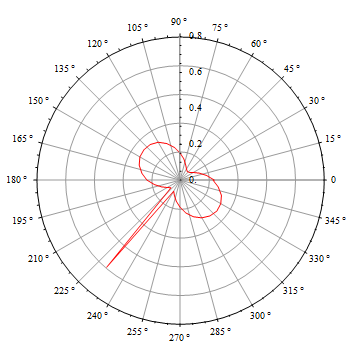
\includegraphics[width=0.45\textwidth]{bilder/1a.png}\\
	\end{tabular}
	\caption{Lineare Polarisation von Weißlicht}
	\label{fig:aufgabe1a}
\end{figure}
\subsubsection{Rotlicht (monochromatisches Licht)}
Indem wir vor der Halogenlampe einen Farbfilter legten, der nur Wellen der Längen zwischen $\unit[630]{nm}$ und $\unit[640]{nm}$ durchlässt, konnten wir monochromatisches (rotes) Licht erzeugen. Die Intensitätsverteilungen entnehmen Sie der Abbildung \ref{fig:aufgabe1b}.
\begin{figure}[H]
	\centering
	\begin{tabular}{@{}r@{}}
		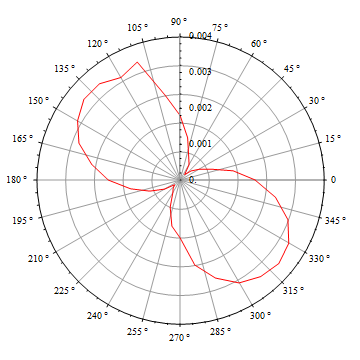
\includegraphics[width=0.45\textwidth]{bilder/1b.png}\\
	\end{tabular}
	\caption{Lineare Polarisation von Rotlicht}
	\label{fig:aufgabe1b}
\end{figure}
Auch wenn nicht sehr genau, man erkennt, dass bei einer Stellung von $\unit[90]{^\circ}$ des Analysators die Intensität fast auf 0 zurückgeht. Dies bedeutet, dass monochromatisches Licht viel besser polarisiert wird, es gibt keine unpolarisierten Anteile. Deshalb wird in den nächsten Versuchen auch durchgehend mit monochromatischem Licht gearbeitet.\\ \\
Auch der Betrag der Intensität ist hier um eine Größenordnung von 100 kleiner, da das meiste Licht vom Farbfilter absorbiert wird.
\subsubsection{Elliptische Polarisation}
Entsprechend der Vorbereitung wurde zum Erzeugen der elliptischen Polarisation ein Glimmerplättchen zwischen Polarisationsfilter und Analysator gebracht. Um die maximale Polarisation zu erreichen, wurde vor der Durchführung des Versuchs eine Kalibrierung vorgenommen, wir suchten zuerst die Stellung des Analysators aus, für die die Intensität minimal wurde und dann drehten wir den Polarisationsfilter um $\unit[45]{^\circ}$. Wir haben die Intensitätsverteilungen für 3 Plättchen verschiedener Dicke gemessen (s. Abbildung \ref{fig:aufgabe1d}, \ref{fig:aufgabe1e} und \ref{fig:aufgabe1f}).
\begin{figure}[H]
	\centering
	\begin{tabular}{@{}r@{}}
		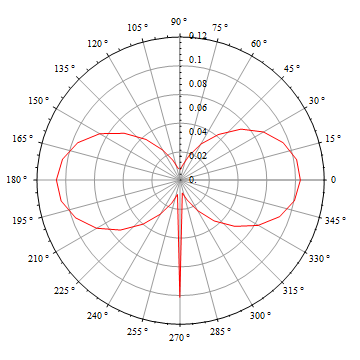
\includegraphics[width=0.4\textwidth]{bilder/1d.png}\\
	\end{tabular}
	\caption{Elliptische Polarisation, Plättchen der Dicke $\unit[45-50]{\mu m}$}
	\label{fig:aufgabe1d}
\end{figure}
\begin{figure}[H]
	\centering
	\begin{tabular}{@{}r@{}}
		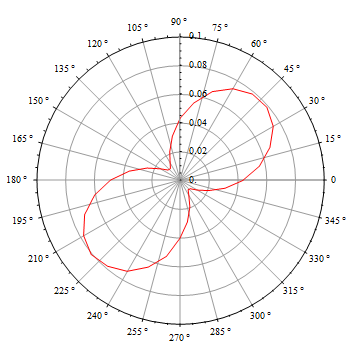
\includegraphics[width=0.4\textwidth]{bilder/1e.png}\\
	\end{tabular}
	\caption{Elliptische Polarisation, Plättchen der Dicke $\unit[52-55]{\mu m}$}
	\label{fig:aufgabe1e}
\end{figure}
Man erkennt anhand der Polardarstellung der Intensitätsverteilungen, dass Licht tatsächlich polarisiert wurde und auch dass bei steigender Dicke der Plättchen die Intensität immer näher zum 0 zurückgeht.
\begin{figure}[H]
	\centering
	\begin{tabular}{@{}r@{}}
		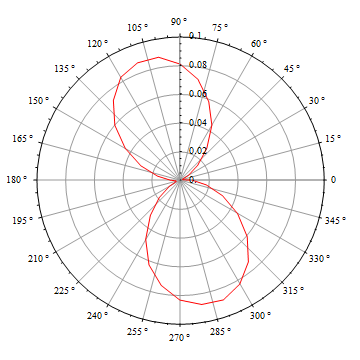
\includegraphics[width=0.45\textwidth]{bilder/1f.png}\\
	\end{tabular}
	\caption{Elliptische Polarisation, Plättchen der Dicke $\unit[60-65]{\mu m}$}
	\label{fig:aufgabe1f}
\end{figure}
\subsubsection{Zirkulare Polarisation}
Mit der zuvor durchgeführten Kalibrierung ersetzten wir das Glimmerplättchen durch ein der Dicke $\frac{\lambda}{4}$ und erhielten die Intensitätsverteilung aus Abbildung \ref{fig:aufgabe1c}. Leider ist es daraus nicht ersichtlich, dass wir hier tatsächlich eine zirkulare Polarisation erzeugten. Die wahrscheinlichste Erklärung dafür liegt an der möglicherweise nicht guten Kalibrierung.
\begin{figure}[H]
	\centering
	\begin{tabular}{@{}r@{}}
		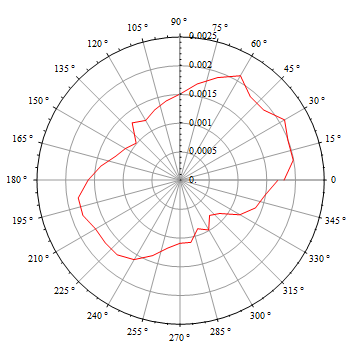
\includegraphics[width=0.45\textwidth]{bilder/1c.png}\\
	\end{tabular}
	\caption{Zirkulare Polarisation, Plättchen der Dicke $\frac{\lambda}{4}$}
	\label{fig:aufgabe1c}
\end{figure}
\section{Aufgabe 2: Differenz der Brechungsindizes}
\begin{enumerate}
\item \textbf{Mit apparativen Daten bei zirkular polarisiertem Licht}
Da die Dicke des $\frac{\lambda}{4}$-Plättchens nicht angegeben war, können wir an dieser Stelle die Brechungsindexdifferenz nicht berechnen.
\item \textbf{Mit der elliptischen Polarisation}
Wir nutzen hierfür die Formel aus der Vorbereitung:
\begin{equation*}
\Delta \phi = 2 \arctan \left( \sqrt{\frac{T}{L}} \right)
\end{equation*}
mit $T$ und $L$ die Taillenweite und Länge der Verteilungsdiagramme.
\begin{table}[H]
\caption{Brechungsindizes der Glimmerplättchen verschiedener Dicken}
\begin{tabular}{c|c|c|c}
	Dicke $d$ in $\mu m$ & $T$ in $V$ & $L$ in $V$ & $\Delta n$ \\
	\hline
	45-50 & 0.0218 & 0.2061 & 0.31 \\
	52-55 & 0.0214 & 0.1618 & 0.35 \\
	60-65 & 0.0069 & 0.1778 & 0.19 \\
\end{tabular}
\label{tab:aufgabe2}
\end{table}
Die Werte der Brechungsindexdifferenzen stimmen in etwa überein, auch wenn die Abweichung für die dickste Platte groß ist. Vielleicht lieg dies daran, dass die Messungen für die dickste Platte unter eventuell veränderten Lichtbedingungen durchgeführt wurden. Trotz unserer Sorgfalt um für möglichst gute Dunkelheit zu sorgen, ergaben sich oft signifikante Abweichungen in den Intensitätsmessungen, wenn wir uns bewegt haben.
\end{enumerate}
\section{Aufgabe 3: Farbänderung bei Drehung des Analysators}
\section{Aufgabe 4: Spannungsdoppelbrechung an Plexiglas}

\end{document}